% Sponge construction diagram for SHA-3/Keccak
% Shows absorb phase (XOR + permute) and squeeze phase (extract + permute)
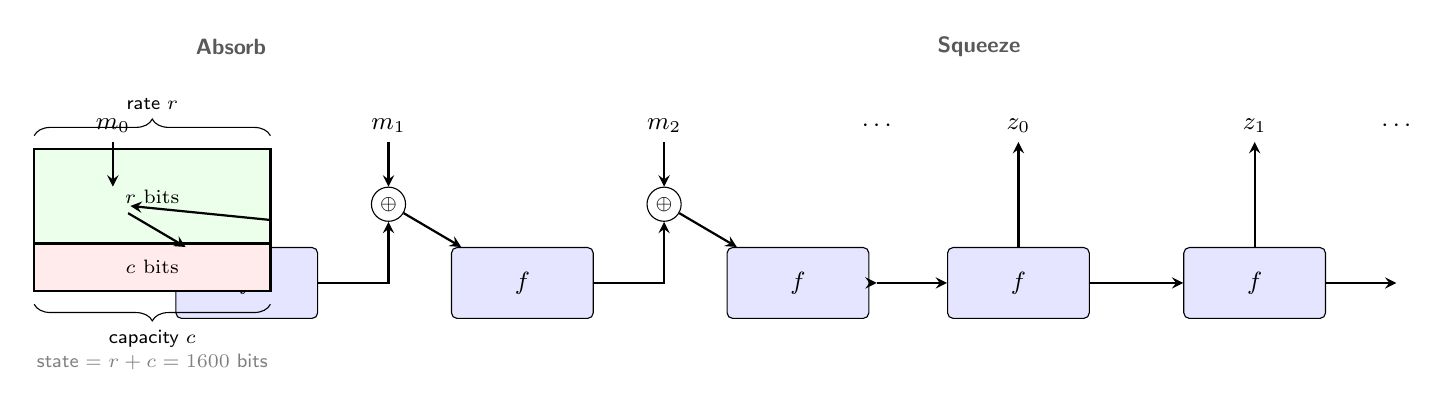
\begin{tikzpicture}[
  >=stealth,
  block/.style={draw, minimum width=1.8cm, minimum height=0.9cm,
                font=\small\sffamily, align=center, rounded corners=2pt},
  xornode/.style={draw, circle, inner sep=1.5pt, font=\scriptsize},
  arr/.style={->, thick},
  brace/.style={decorate, decoration={brace, amplitude=6pt, raise=2pt}},
  label/.style={font=\footnotesize\sffamily, text=gray!70!black}
]

% State representation
\def\stateW{3.0}
\def\rateH{1.2}
\def\capH{0.6}

% --- Absorb phase ---
\node[label] at (0, 2.5) {\textbf{Absorb}};

% Input blocks
\node[font=\small] (m0) at (-1.5, 1.5) {$m_0$};
\node[font=\small] (m1) at (2.0, 1.5) {$m_1$};
\node[font=\small] (m2) at (5.5, 1.5) {$m_2$};
\node[font=\small] (dots) at (8.2, 1.5) {$\cdots$};

% XOR nodes
\node[xornode] (xor0) at (-1.5, 0.5) {$\oplus$};
\node[xornode] (xor1) at (2.0, 0.5) {$\oplus$};
\node[xornode] (xor2) at (5.5, 0.5) {$\oplus$};

% Permutation blocks
\node[block, fill=blue!10] (f0) at (0.2, -0.5) {$f$};
\node[block, fill=blue!10] (f1) at (3.7, -0.5) {$f$};
\node[block, fill=blue!10] (f2) at (7.2, -0.5) {$f$};

% State boxes (rate + capacity)
\draw[thick, fill=green!8] (-2.5, 0.0) rectangle (-2.5+\stateW, \rateH);
\node[font=\scriptsize] at (-2.5+\stateW/2, \rateH/2) {$r$ bits};
\draw[thick, fill=red!8] (-2.5, -\capH) rectangle (-2.5+\stateW, 0.0);
\node[font=\scriptsize] at (-2.5+\stateW/2, -\capH/2) {$c$ bits};

% Arrows: input to XOR
\draw[arr] (m0) -- (xor0);
\draw[arr] (m1) -- (xor1);
\draw[arr] (m2) -- (xor2);

% Arrows: XOR to f
\draw[arr] (xor0) -- (f0);
\draw[arr] (xor1) -- (f1);
\draw[arr] (xor2) -- (f2);

% Arrows: f to next XOR
\draw[arr] (f0) -| (xor1);
\draw[arr] (f1) -| (xor2);
\draw[arr] (f2) -- (8.2, -0.5);

% Initial state arrow
\draw[arr] (-2.5+\stateW, 0.3) -- (xor0);

% --- Squeeze phase ---
\node[label] at (9.5, 2.5) {\textbf{Squeeze}};

\node[block, fill=blue!10] (fs0) at (10.0, -0.5) {$f$};
\node[block, fill=blue!10] (fs1) at (13.0, -0.5) {$f$};

% Output blocks
\node[font=\small] (z0) at (10.0, 1.5) {$z_0$};
\node[font=\small] (z1) at (13.0, 1.5) {$z_1$};
\node[font=\small] (zdots) at (14.8, 1.5) {$\cdots$};

% Arrows: f to output
\draw[arr] (fs0) -- (z0);
\draw[arr] (fs1) -- (z1);

% Arrows: chain
\draw[arr] (8.2, -0.5) -- (fs0);
\draw[arr] (fs0) -- (fs1);
\draw[arr] (fs1) -- (14.8, -0.5);

% Rate/capacity annotation
\draw[brace] (-2.5, \rateH+0.1) -- node[above=8pt, font=\scriptsize\sffamily]
  {rate $r$} (-2.5+\stateW, \rateH+0.1);
\draw[brace] (-2.5+\stateW, -\capH-0.1) -- node[below=8pt, font=\scriptsize\sffamily]
  {capacity $c$} (-2.5, -\capH-0.1);

% Annotation: state width
\node[font=\scriptsize\sffamily, text=gray] at (-1.0, -1.5)
  {state = $r + c = \num{1600}$ bits};

\end{tikzpicture}
